\documentclass[10pt]{article}
\usepackage{icmlko}

\icmlmeta{IP 파운데이션 월드모델}{165}{슬롯에 세 들어 있던 손잡이}{노트 164가 ``제작사 이력을 여섯째 축으로 세우면''을 남겼다. 세워 봤더니 그 세입자가 집주인보다 나은 손잡이인데, 집을 나가면 판이 내려간다}

\begin{document}

\twocolumn[
\icmlheader

\begin{abstract}
노트 164가 \texttt{venue\_prominence} 슬롯이 열 도메인 중 일곱에서 실은
``제작사/개발사의 사전 출시작 수''임을 코드로 확인하고, ``여섯째 축으로
따로 세우면''을 남겼다. 두 가지로 세워 봤다 --- \textbf{분리}(일곱 도메인의
값을 새 축으로 \emph{옮기고} 장소 슬롯을 비운다)와 \textbf{복제}(슬롯은
그대로 두고 새 축을 \emph{더한다}). 결과가 셋이다.
\textbf{① 분리하면 판이 내려간다.} F18 배깅이 $+$0.4465에서 $+$0.4343으로,
격차 $+$0.0122 $\pm$ 0.0030($t{=}4.1$)로 \textbf{갈린다}. 슬롯을 일곱
도메인이 나눠 쓰는 것이 \emph{구성물이 달라도} 값을 하고 있었다 --- 노트
139의 ``풀링은 지켜 준다''를 슬롯 수준에서 잰 셈이다.
\textbf{② 그런데 그 세입자가 집주인보다 나은 손잡이다.} 새 축
\texttt{creator\_track} 의 사전 부호 일치가 \textbf{5/5} 다 --- 두 정식화
모두, 채점되는 다섯 도메인 전부. 반면 순수해진 장소 노출은 남은 두 칸에서
F18 1/2 · F6 0/2로 무너진다.
\textbf{③ 복제는 공선성을 만든다.} 판은 안 움직이는데($-$0.0029 $\pm$
0.0018, $t{=}1.6$) 단순 부호 일치가 F6 에서 89\%에서 \textbf{73\%}로
떨어진다 --- 같은 열이 둘이면 능형이 계수를 갈라 갖고 원래 축의 방향이
흐려진다. \textbf{그래서 배선은 안 바꾼다.} 셋 다 판에서 손해거나
무의미하고, 손잡이 쪽 이득은 새 축 하나뿐이다. 남기는 것은 사실 하나다 ---
\textbf{이 판에서 제일 깨끗하게 움직이는 구성물은 지금까지 이름이 없던
것이다.} 제작사의 사전 출시작 수는 일곱 도메인이 공유하고, 다섯 칸 전부
옳은 방향으로 움직이며, 지금은 ``장소 노출''이라는 남의 이름으로 불린다.
\end{abstract}
]

\begin{figure*}[t]
\centering
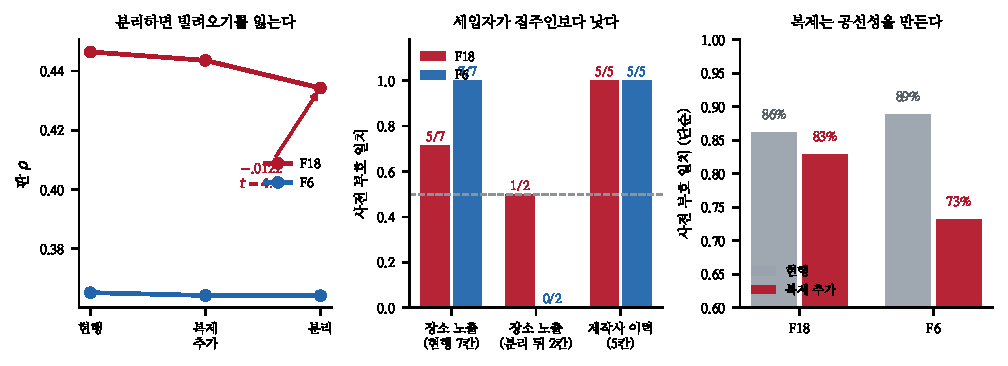
\includegraphics[width=\textwidth]{figs/tenant.pdf}
\caption{왼쪽 --- 분리하면 빌려오기를 잃는다. 가운데 --- 세입자가 집주인보다
낫다. 오른쪽 --- 복제는 공선성을 만든다.}
\end{figure*}

\section{분리하면 판이 내려간다}

\begin{table}[t]
\centering\tsize
\caption{판 $\rho$. 팝업 방향 보정은 노트 160대로 뺀 상태.}
\begin{tabular}{lrrrr}
\toprule
& \multicolumn{2}{c}{F18 배깅} & \multicolumn{2}{c}{F6 능형} \\
& 판 & 팝업 & 판 & 팝업 \\
\midrule
현행 & \textbf{$+$.4465} & $+$.3388 & \textbf{$+$.3651} & $+$.4286 \\
복제 추가 & $+$.4436 & $+$.3301 & $+$.3642 & $+$.4014 \\
\textbf{분리} & \textbf{$+$.4343} & $+$.3621 & $+$.3641 & $+$.4008 \\
\bottomrule
\end{tabular}
\end{table}

\claimx{\textbf{분리가 F18 에서 $+$0.0122 $\pm$ 0.0030($t{=}4.1$)로
갈린다.} 슬롯을 일곱 도메인이 나눠 쓰는 것이 \emph{구성물이 달라도} 값을
하고 있었다.}{노트 139가 잰 ``풀링은 지켜 주고 희석한다''를 슬롯 수준에서
본 것이다. 다른 물건을 같은 칸에 넣어도 빌려오기는 작동한다 --- 그것이
좋은 설계라는 뜻은 아니고, \textbf{지금 판이 그 빌려오기에 기대고 있다}는
뜻이다.}

\claimx{\textbf{복제는 판을 안 건드린다}($-$0.0029 $\pm$ 0.0018,
$t{=}1.6$).}{옮기지 않고 더하기만 했으니 당연하다. 문제는 다른 데서 난다.}

\section{세입자가 집주인보다 낫다}

\begin{table}[t]
\centering\tsize
\caption{사전 부호 일치.}
\begin{tabular}{lrr}
\toprule
& F18 & F6 \\
\midrule
장소 노출 (현행 7칸) & 5/7 & 7/7 \\
장소 노출 (분리 뒤 2칸) & 1/2 & \textbf{0/2} \\
\textbf{제작사 이력 (5칸)} & \textbf{5/5} & \textbf{5/5} \\
\bottomrule
\end{tabular}
\end{table}

\claimx{\textbf{\texttt{creator\_track} 은 5/5 다} --- 두 정식화, 채점되는
다섯 도메인 전부. 노트 163이 잰 타깃 폭(45/45) · 굿즈 규모(39/40)와 같은
급이다.}{다섯 칸뿐이라 5/5의 표준오차가 크다($p{=}0.9$ 여도 $5/5$ 가 나올
확률이 59\%다). 다만 두 정식화가 독립적으로 5/5 라는 것이 조금 더 센 증거다.}

\claimx{\textbf{순수해진 장소 노출은 무너진다}(F18 1/2 · F6 0/2). 남는
도메인이 둘뿐이라 잴 것이 없다.}{현행 7/7(F6)이 좋아 보였던 것은 대부분
제작사 이력이 낸 성적이었다 --- 일곱 칸 중 다섯이 그것이다.}

\section{복제는 공선성을 만든다}

\begin{table}[t]
\centering\tsize
\caption{단순 부호 일치.}
\begin{tabular}{lrr}
\toprule
& 현행 & 복제 추가 \\
\midrule
F18 배깅 & 86\% & 83\% \\
\textbf{F6 능형} & \textbf{89\%} & \textbf{73\%} \\
\bottomrule
\end{tabular}
\end{table}

\claimx{\textbf{옳은 칸 다섯을 더했는데 비율이 내려간다.} 같은 열이 둘이면
능형이 계수를 갈라 갖고, 원래 \texttt{venue\_prominence} 의 방향이
흐려진다. 트리는 덜 영향받는다(86\%$\to$83\%).}{``정보를 더 줬으니
나빠질 리 없다''가 틀리는 자리다. \textbf{같은 정보를 두 번 주면
해석이 나빠진다} --- 예측은 그대로여도.}

\section{그래서 배선은 안 바꾼다}

\begin{table}[t]
\centering\tsize
\caption{셋의 대차대조.}
\begin{tabular}{lll}
\toprule
& 판 & 손잡이 \\
\midrule
현행 & 기준 & 장소 7/7(F6) --- 실은 제작사 \\
복제 & 무의미 & 새 축 5/5, 원래 축 흐려짐 \\
분리 & \textbf{$-$.0122} & 새 축 5/5, 장소 0/2 \\
\bottomrule
\end{tabular}
\end{table}

\claimx{\textbf{셋 다 안 채택한다.} 판에서 손해거나 무의미하고, 손잡이 쪽
이득은 새 축 하나뿐인데 그것도 다섯 칸이다.}{노트 164가 세운 규약(``슬롯
이름이 아니라 구성물을 맞춘다'')은 \emph{새 도메인을 붙일 때}의 규약으로
남긴다. \textbf{이미 붙은 것을 되돌리는 것은 다른 문제고, 이 노트가 그
값을 쟀다 --- $-$0.0122 다.}}

\begin{table}[t]
\centering\tsize
\caption{남은 것.}
\begin{tabular}{ll}
\toprule
\textbf{이름} & 제일 깨끗한 구성물에 이름이 없다 \\
빌려오기 & 구성물이 달라도 되는 이유 --- 순위만 쓰기 때문? \\
다섯 칸 & creator\_track 을 게임·애니·웹툰에도 붙이면 \\
\bottomrule
\end{tabular}
\end{table}

마지막 줄이 값싸다. 게임은 이미 개발사 사전작을 세는데 마스크가 0이고,
애니 · 웹툰은 스튜디오 · 요일을 쓰고 있다. 셋에 제작사 사전작을 붙이면
칸이 다섯에서 여덟이 되고, \textbf{5/5가 우연인지 아닌지 갈린다.}

\end{document}
